% !TeX root = ./report.tex

\documentclass{IEEEtran}
\usepackage{bm}
\usepackage{amsmath}
\usepackage{amssymb}
\usepackage{booktabs}
\usepackage{algorithm}
\usepackage{algorithmicx}
\usepackage{algpseudocode}
\usepackage{footnote}
\usepackage{stfloats}
\usepackage{graphicx}
\usepackage{url}
\DeclareMathOperator*{\argmax}{arg\,max}
\DeclareMathOperator*{\argmin}{arg\,min}
\makesavenoteenv{figure}
\title{Title}
\author{
    Fan~JIN
    \thanks{Fan~JIN 2015011506  \texttt{jinf15@mails.tsinghua.edu.cn}}
}

\begin{document}
\maketitle
\begin{abstract}
    Abstract
\end{abstract}
\begin{IEEEkeywords}
    Keywords 1, Keywords 2,
\end{IEEEkeywords}

\section{Question 1: Function Optimization}
{
    \subsection{Target function: Eggholder}
    {
        As intelligent optimization algorithms have emerged as a new paradigm of function optimization, 
        many test functions have been proposed to serve as benchmarks \cite{wiki:Test_functions_for_optimization}.
        In this report, the Eggholder function is chosen to test two intelligent optimization algorithms:
        the simulated annealing (SA) and the differential evolution (DE).

        The Eggholder function is defined as
        \[
            \begin{split}
            f(x,y) &= \\
            &- (y+47) \sin{\sqrt{\left| \frac{x}{2}+(y+47) \right|}} \\
            &- x \sin{\sqrt{\left| x-(y+47) \right|}},
            \end{split}
        \]
        where $-512 < x,y < 512$.
        Its global minimum is known as $f(512, 404.2319) = -959.6407$.

        \begin{figure}[!htbp]
            \centering
            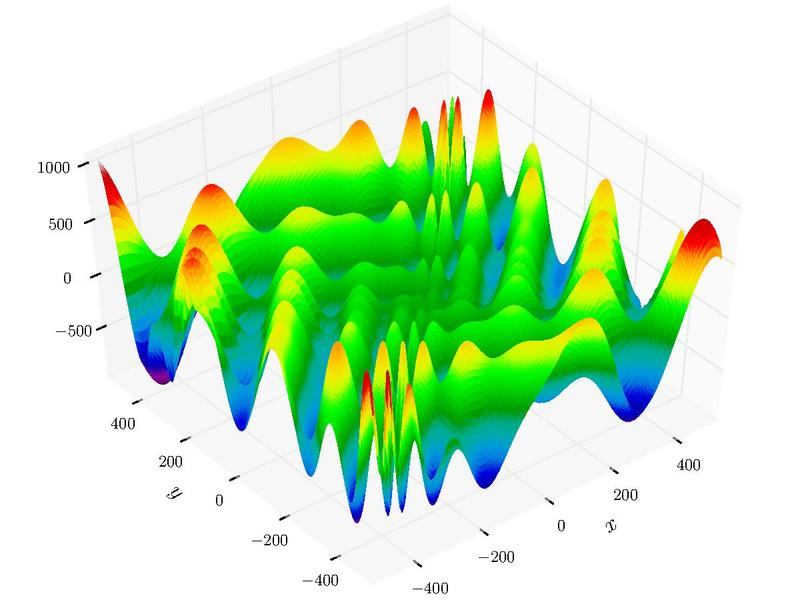
\includegraphics[width=0.45\textwidth]{figures/eggholder.png}
            \caption{Eggholder function \cite{wiki:Test_functions_for_optimization}}
            \label{fig:eggholder}
        \end{figure}

        Eggholder function is challenging bacause 
        i) it has boundary constraints on both $x$ and $y$, and 
        ii) the global minimum is at the boundary of $x=512$, and 
        iii) there are dozens of local minimums throughout the space.
        
    }
}

\bibliographystyle{ieeetran}
\bibliography{reference}
\end{document}